\documentclass[letterpaper,12pt]{article}
\usepackage{tabularx} % extra features for tabular environment
\usepackage{amsmath}  % improve math presentation
\usepackage{graphicx} % takes care of graphic including machinery
\usepackage[margin=1in,letterpaper]{geometry} % decreases margins
\usepackage{wrapfig, blindtext}
\usepackage{graphicx}
\usepackage{placeins}
\usepackage{cite} % takes care of citations
\usepackage[final]{hyperref} % adds hyper links inside the generated pdf file
\hypersetup{
	colorlinks=true,       % false: boxed links; true: colored links
	linkcolor=blue,        % color of internal links
	citecolor=blue,        % color of links to bibliography
	filecolor=magenta,     % color of file links
urlcolor=blue}
%\FloatBarrier


\begin{document}
\title{}
\author{}
\date{}
%


\begin{center}
\textbf{Lane Finding - Jack Wetherell} \\
\end{center}


\section{Pipeline}
My computer vision (CV) pipeline takes a single image as an input, and returns the image with the left and right lanes annotated, along with several images taken at the end of each stage of the pipeline, for development and visualisation purposes. This pipeline correctly annotates the given example images and videos, but has several shortcomings and possible improvements. My CV pipeline contains the following stages (values of all hyper-parameters are detailed in the notebook):
\begin{enumerate}
\item \textbf{Gray-scaling}\\
Firstly the image is converted to gray scale, reducing the dimensionality of the image from $(X,Y,3)$ to $(X,Y,1)$, where $X$ and $Y$ are the number of pixels in each dimension of the image. I use openCV to perfrom this conversion, which utilises the following conversion convention: $G= 0.299r + 0.587g + 0.114b$.
\item \textbf{Blurring}\\
The next stage is to blur the image using a Gaussian Blur filter. I chose a kernel size of 5x5. This stage ensures that the pipeline is resistant to high frequency noise present in the image.
\item \textbf{Canny Edge Detection}\\
The next stage in the pipeline is to apply Canny edge detection. This first computes the derivative of the image in the $x$ and $y$ directions, and takes the Pythagorean sum to determine the total derivative at each point. The pixels that have the most neighbours are then selected the be the 'centre' pixels. The resultant image contains a 2 value array image, where the detected lines are shown.
\item \textbf{Mask Application}\\
As the edge detection image finds all edges in the image, we need to apply a mask to the image to only show the lines that correspond to lane lines. I use a 4 point polygon to only select the edges that correspond to the lane lines.
\item \textbf{Hough Transform}\\
The next stage is to use a Hough transform to detect the lines in the image. This is performed using the open CV implementation. This function returns a list of pairs of points the form lines in the image. In the first instance I simply use these lines to annotate the image. This results in the annotation not being able to treat dashed lane lines as continuous. \textit{Below I go into detail of how I adjust the method to solve this problem.}
\item \textbf{Annotation}\\
Finally the set of lines as described by the pairs of points are drawn to the image as semi-transparent red lines. 

\end{enumerate}
Each stage of this process is shown in the following figure. Each column shows each stage of the pipeline applied to each of the given test images:
\FloatBarrier
\begin{figure}
\centering
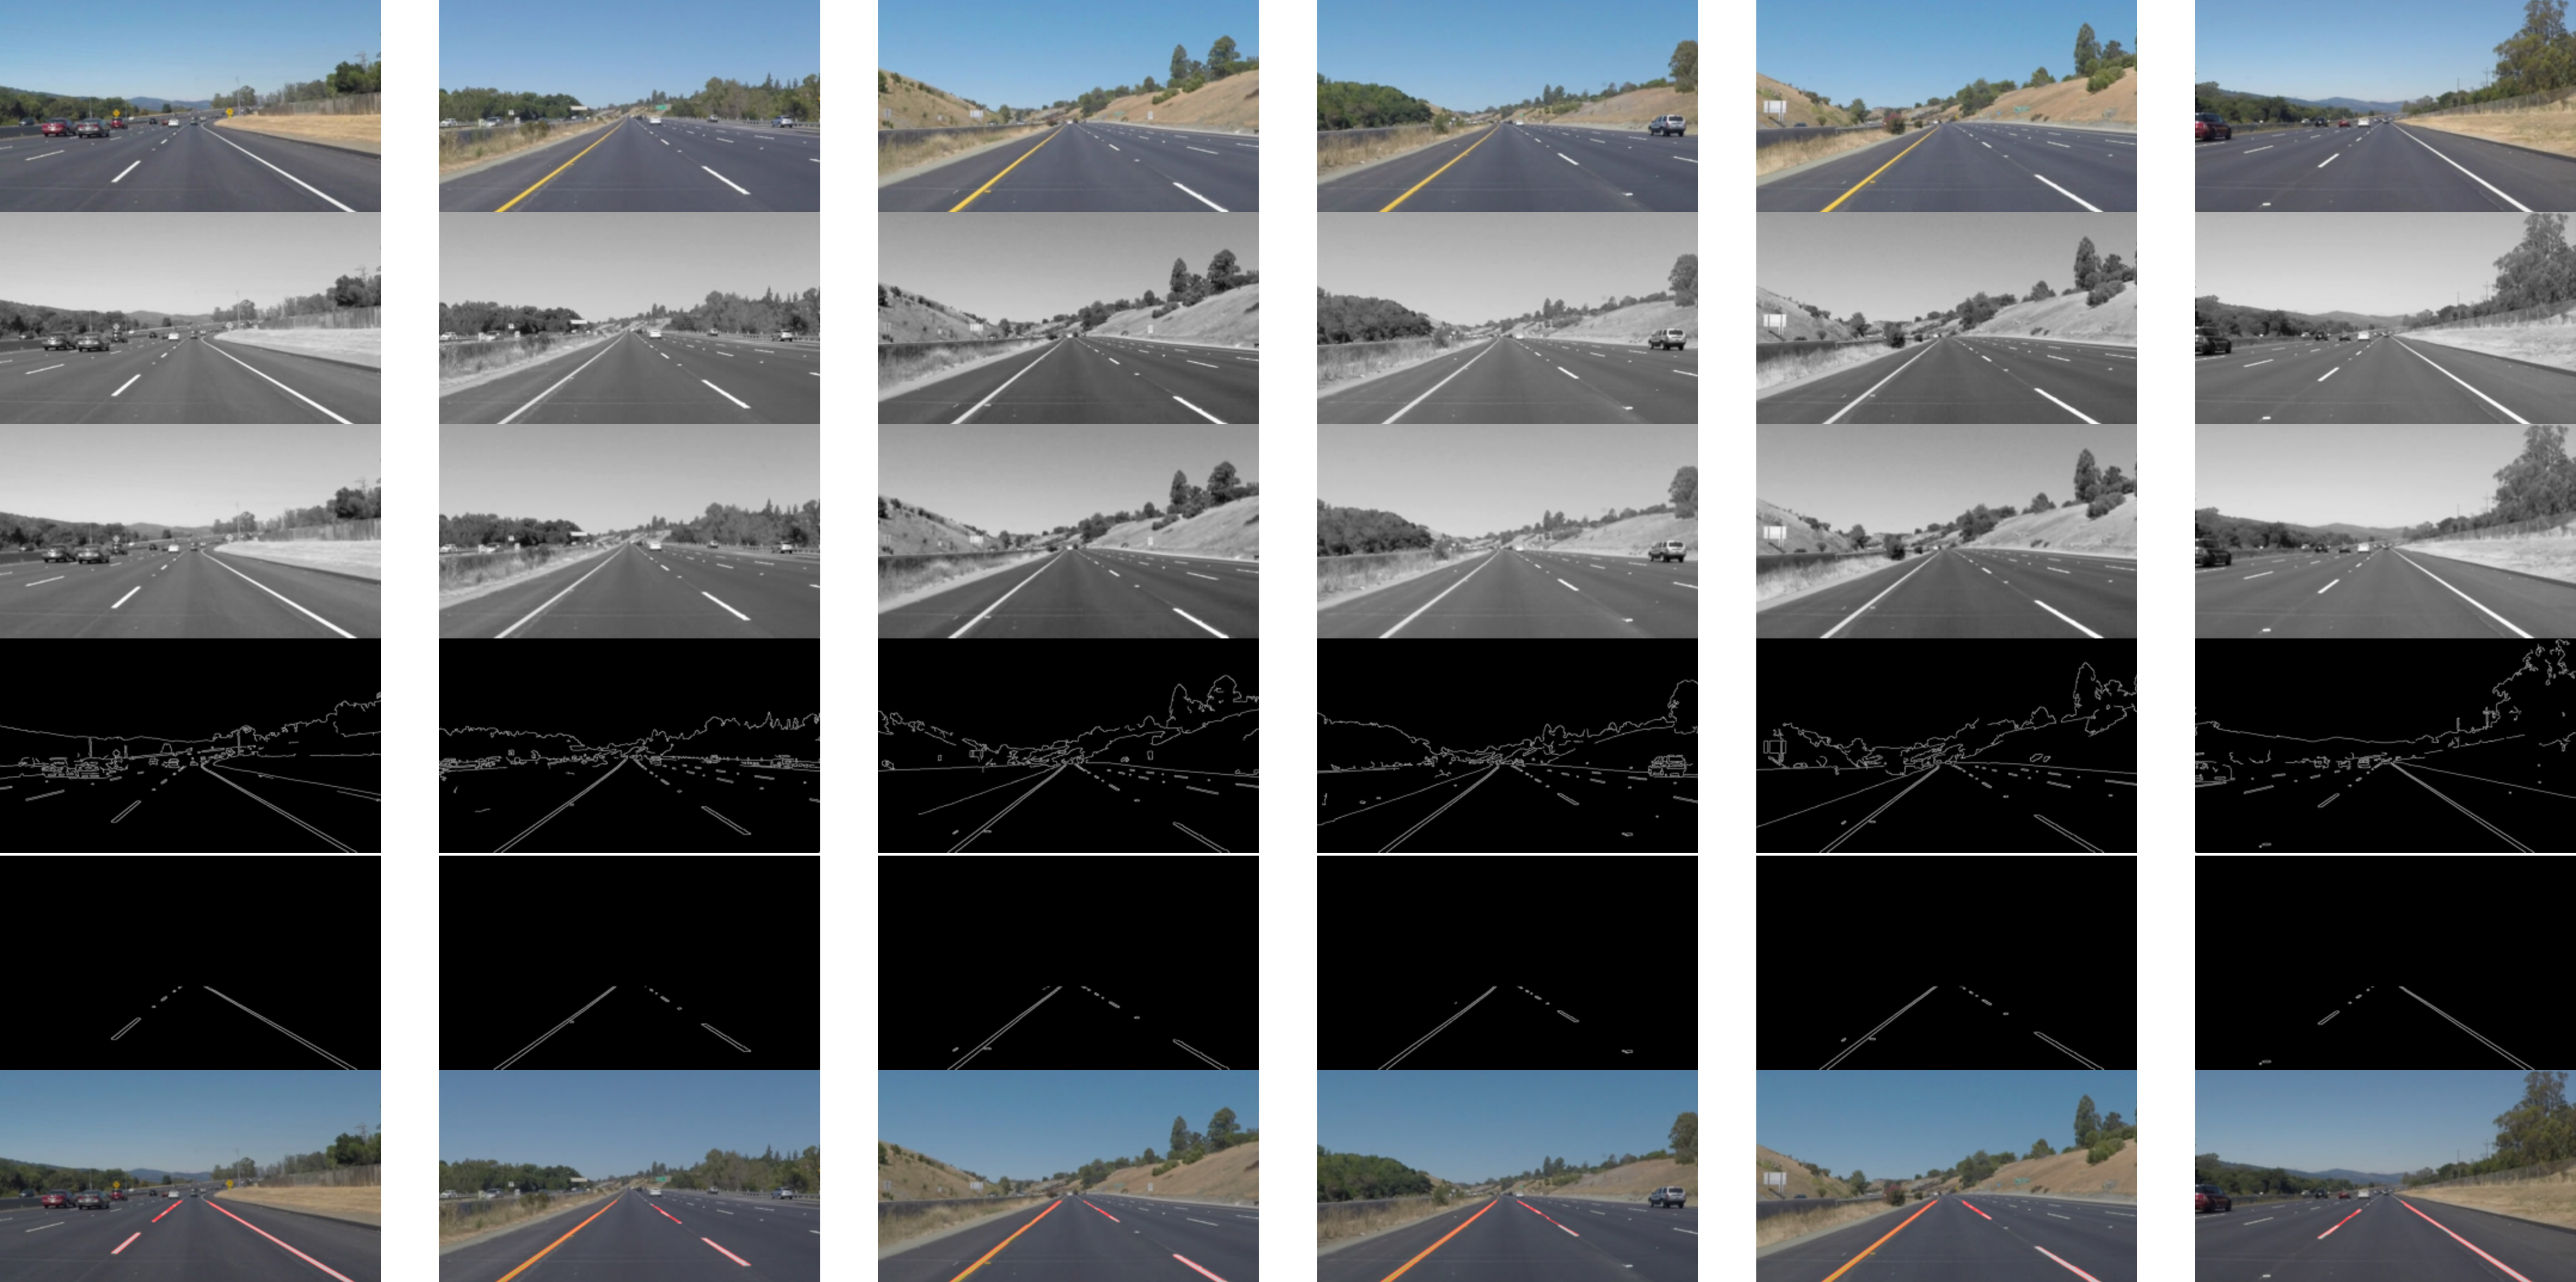
\includegraphics[width=0.9\columnwidth]{fig1_clean.pdf}
\label{fig:figure}
\end{figure}
\FloatBarrier
\noindent As can be seen, the non-continous road markings are also non-continous in the annotation. This is not desirable as we simply want to determine where the lane lines are, in order to determine where the car is relative to the lane markings. In order to fix this I insert a sub-pipleine into the CV pipeline. This takes the lines found by the Hough transform in stage 5. And filters the lines to only 2 lines: one for the left and right lanes respectively. This is achieved in the following stags:
\begin{enumerate}

 \item \textit{Gradient Separation}\\
The first stage is to separate the set of lines into two buckets: left and right lines. This is achieved by separating the lines based on the sign of the gradient.  Positive for the left lane lines, and negative for the right. This is due to the consistent parallax effect in the camera images. In addition, I also only include lines whose absolute gradient is greater then 0.5, this means that other markings on the road perpendicular to travel are filtered out at this stage.
 \item \textit{Linear Fitting}\\
Now for each of the two buckets of lines, I simply treat them as two sets of points, and use scipy's \textit{curve fit} function to fit a straight line to each. This gives a description of the two lines, given by a gradient and y-intercept. I then determine the end points of this line that fit within the previously described mask, yielding 4 endpoints, two for each lane. These two descriptions of the two lines is then passed to step 6 of the main CV pipeline.
\end{enumerate}

\noindent When applied to the test image, this fixes the problem, and now both the left and right lanes are annotated as continuous lines, regardless of if they are actually continuous on the road. This improvement is shown in the figure below:
\FloatBarrier
\begin{figure}
\centering
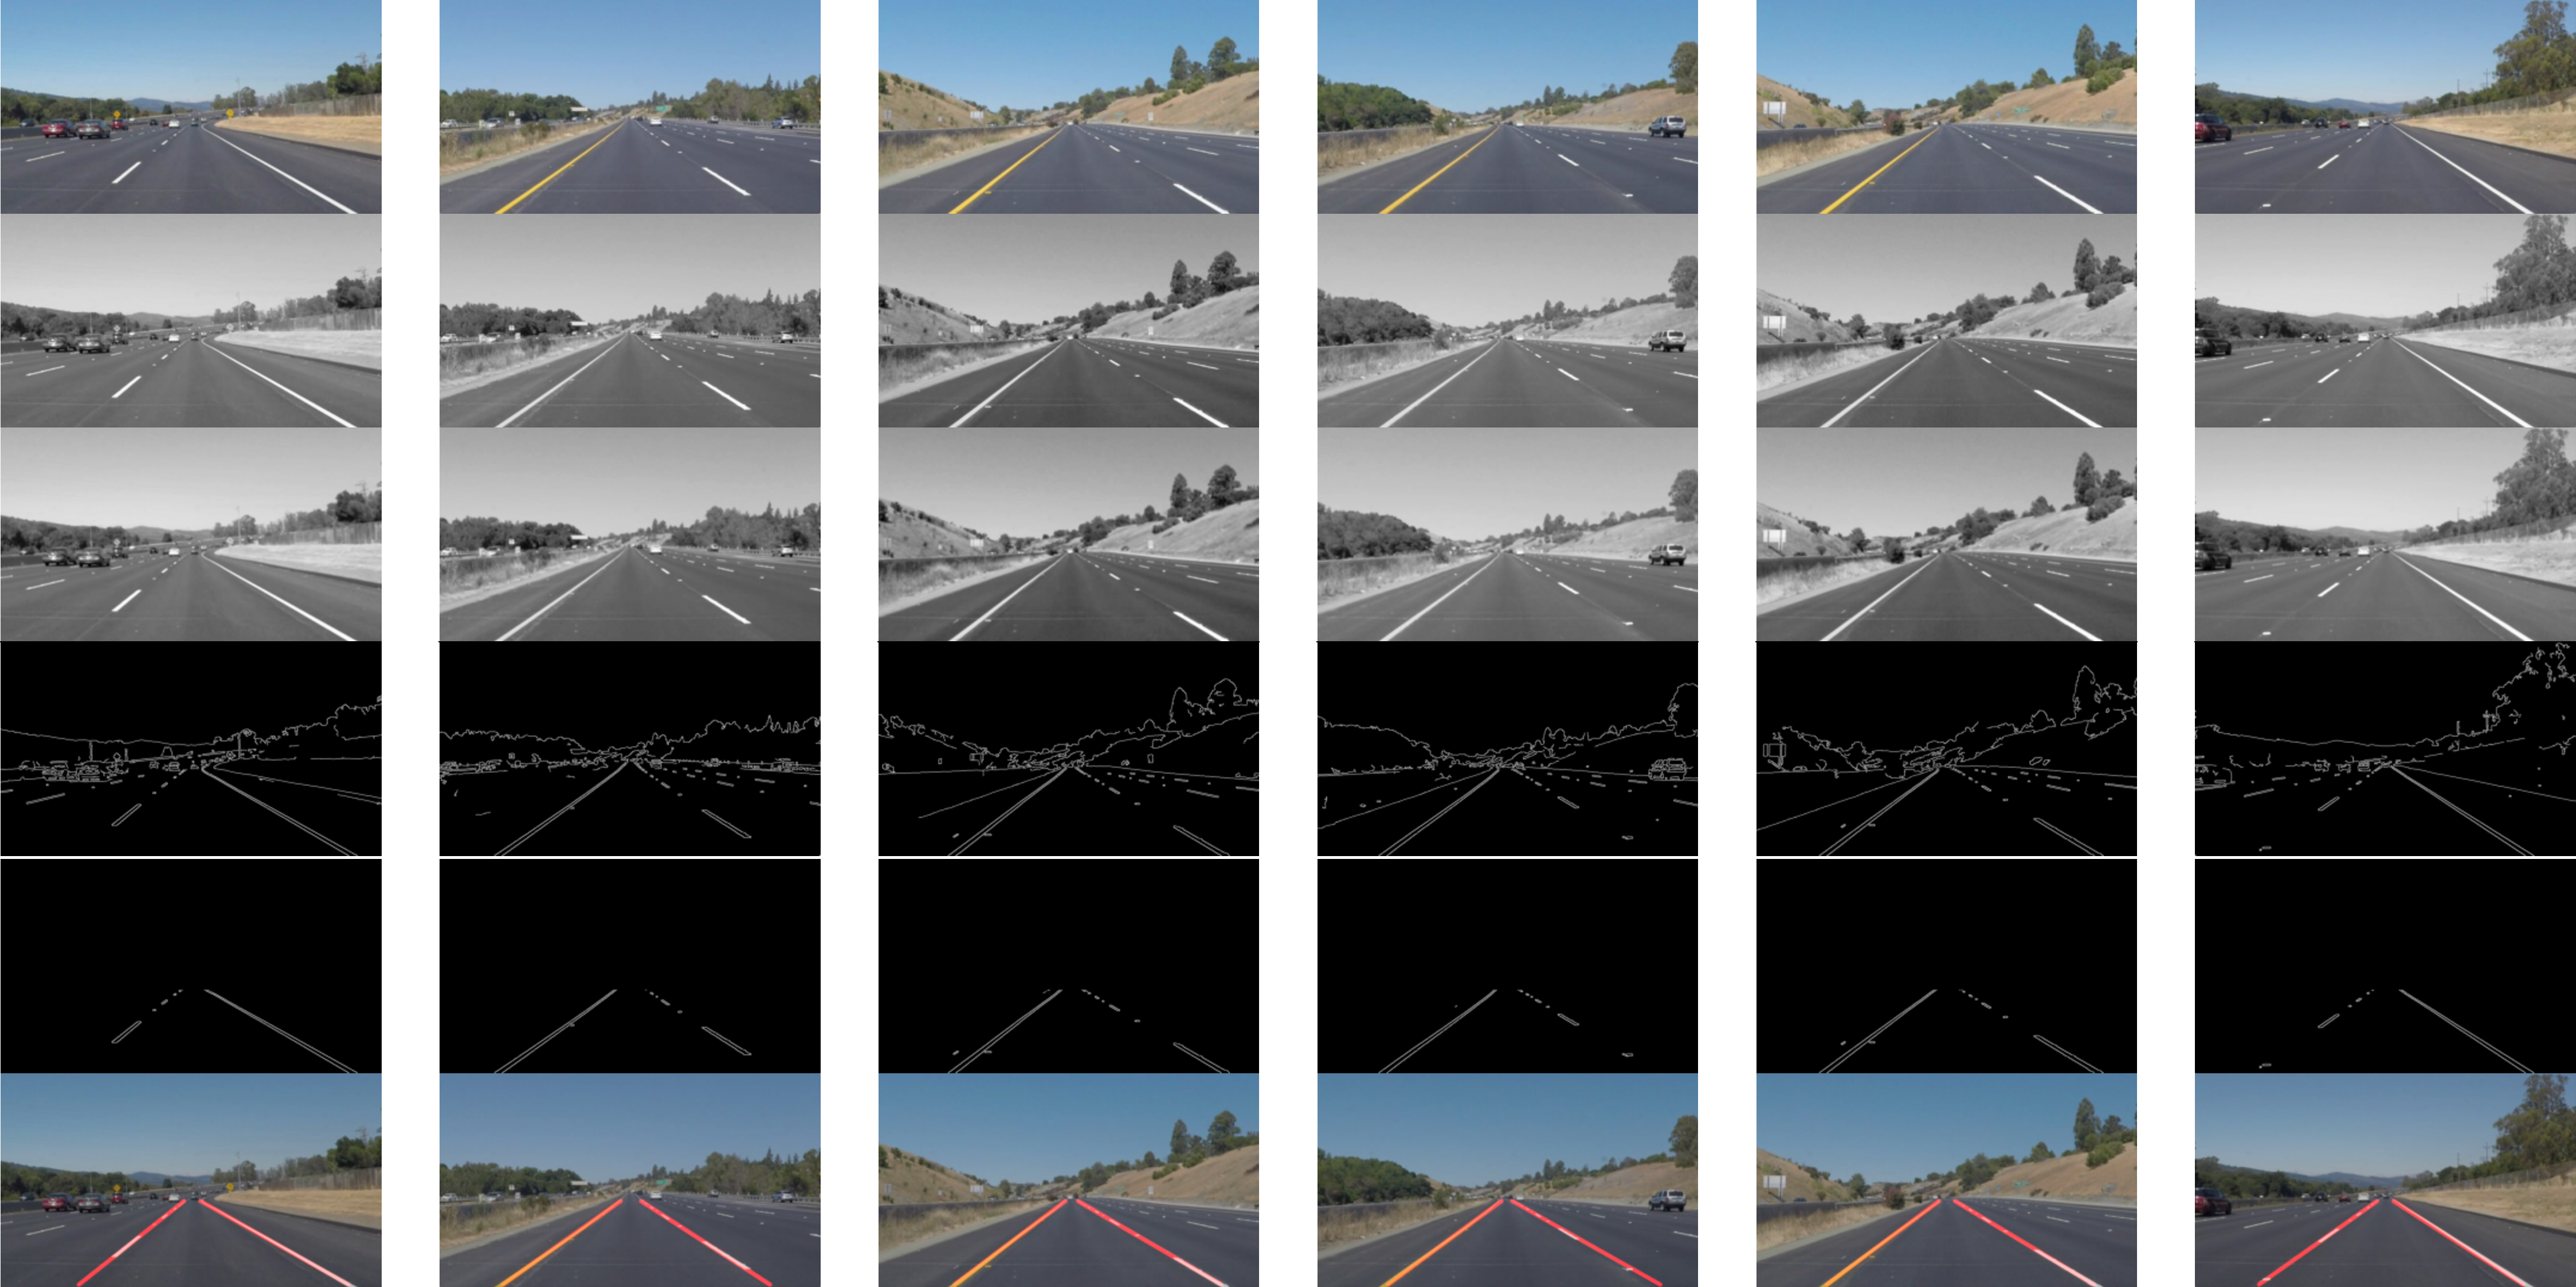
\includegraphics[width=1.0\columnwidth]{fig2_clean.pdf}
\label{fig:figure}
\end{figure}
\FloatBarrier

This correctly annotates the lanes in the two given video examples accurately (results shown in the notebook).
\section{Shortcomings}
This CV pipeline has the following shortcomings:
\begin{enumerate}
\item It assumes a given position of where the camera is mounted on the front of the vehicle. If this were to change the parameters defining the mask would likely no longer be appropriate.
\item It is not fully resistant to shadows on the road, that if they have the appropriate gradient in the image, could cause the CV pipeline to incorrectly classify the shadow as part of the lane.
\item It is only designed to work with straight road lanes, it will not be effective on significantly curved roads.
\item Due to the gradient separation stage, this would not be effective during the transition of lane changing.
\end{enumerate}
I suggest an possible improvements that could ameliorate these shortcomings in the following section:

\section{Improvements}
I suggest the following improvements to the pipeline, for each of the shortcomings discussed above:
\begin{enumerate}
\item One possible improvement to rectify this issue is a method inspired by the Monte Carlo integration method. One would choose many masks randomly distributed around a default mask, the masks the produces the most stable lane lines (most agreement, based on the gradient of the resultant lines falling in some given desirable range) would be selected and averaged.
\item This could be rectified by removing points in the \textit{draw lines} routine that fall outside a given standard deviation, as these are unlikely to be lane lines.
\item The threshold of the length of lines could be adjusted in the Hough transform such that a curved lines is seen as many shorted straight lines. These points could then be fitted, assuming the fit function was modified from a linear function to a second order polynomial. This would allow the method to detect and annotated curved lanes.
\item This could be solved by using extrapolation based on earlier frames in the video, as the transition over the lane occurs. This would of course mean the method could not be applied to individual frames, but instead a series of frames in a video segment.
\end{enumerate}


\end{document}